\section{Ease of use}
\label{sec:Ease}
Using the command line we can execute the program using one of these options:\\


\begin{figure}[H]
   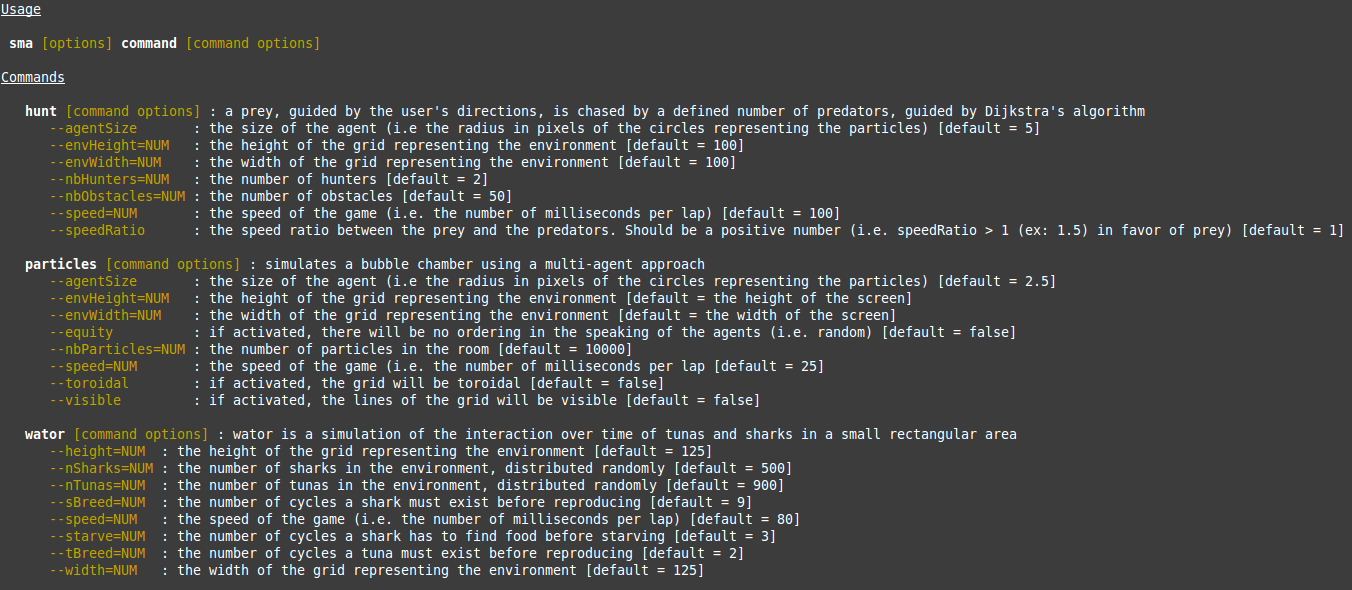
\includegraphics[width=\linewidth]{usage.png}
   \caption{Usage}
\end{figure}



Example of executing the command line with default parameters:
\begin{lstlisting}[language=bash]
  $ java -jar target/scala-2.11/scalagent.jar hunt
\end{lstlisting}

Example of executing the command line with specific parameters:
\begin{lstlisting}[language=bash]
  $ java -jar target/scala-2.11/scalagent.jar particles --nbParticles=15000 --toroidal=true
\end{lstlisting}